%%%%%%%%%%%%%%%%%%%%%%%%%%%%%%%%%%%%%%%%%
% Stylish Article
% LaTeX Template
% Version 2.1 (1/10/15)
%
% This template has been downloaded from:
% http://www.LaTeXTemplates.com
%
% Original author:
% Mathias Legrand (legrand.mathias@gmail.com) 
% With extensive modifications by:
% Vel (vel@latextemplates.com)
%
% License:
% CC BY-NC-SA 3.0 (http://creativecommons.org/licenses/by-nc-sa/3.0/)
%
%%%%%%%%%%%%%%%%%%%%%%%%%%%%%%%%%%%%%%%%%

%----------------------------------------------------------------------------------------
%	PACKAGES AND OTHER DOCUMENT CONFIGURATIONS
%----------------------------------------------------------------------------------------

\documentclass[fleqn,12pt]{SelfArx} % Document font size and equations flushed left

\usepackage[english]{babel} % Specify a different language here - english by default

\usepackage{lipsum} % Required to insert dummy text. To be removed otherwise

\captionsetup[figure]{justification=justified, singlelinecheck=off} 
\captionsetup[table]{justification=justified, singlelinecheck=off} 

%----------------------------------------------------------------------------------------
%	COLUMNS
%----------------------------------------------------------------------------------------

\setlength{\columnsep}{0.55cm} % Distance between the two columns of text
\setlength{\fboxrule}{0.75pt} % Width of the border around the abstract
\linespread{1.5}

%----------------------------------------------------------------------------------------
%	COLORS
%----------------------------------------------------------------------------------------

\definecolor{color1}{RGB}{0,0,90} % Color of the article title and sections
\definecolor{color2}{RGB}{10,20,20} % Color of the boxes behind the abstract and headings
\definecolor{xsubj}{RGB}{243,194,68} 
\definecolor{xsess}{RGB}{53,99,161} 
\definecolor{xsamp}{RGB}{18,165,121} 

%----------------------------------------------------------------------------------------
%	HYPERLINKS
%----------------------------------------------------------------------------------------

\usepackage{hyperref} % Required for hyperlinks
\hypersetup{hidelinks,colorlinks,breaklinks=true,urlcolor=color2,citecolor=color1,linkcolor=color1,bookmarksopen=false,pdftitle={Title},pdfauthor={Author}}

%----------------------------------------------------------------------------------------
% Macros that fit better here than the template
%----------------------------------------------------------------------------------------
\makeatletter
\let\Hy@linktoc\Hy@linktoc@none

\let\l@secnonum\l@section
\newcounter{secnonum}
\renewcommand{\thesecnonum}{}

\let\l@supsec\l@section
\newcounter{supsec}
\renewcommand{\thesupsec}{Ch.0 - S\arabic{supsec}}%

\titleclass{\secnonum}{straight}[\section]
\setcounter{secnumdepth}{5}
\titleformat{\secnonum}
  {}{}{}{}
\titlespacing*{\secnonum}{0pt}{}{}

\titleclass{\supsec}{straight}[\section]
\titleformat{\supsec}
  {}{}{}{}
\titlespacing*{\supsec}{0pt}{}{}

\makeatother

%----------------------------------------------------------------------------------------
%	ARTICLE INFORMATION
%----------------------------------------------------------------------------------------

% \JournalInfo{Journal, Vol. XXI, No. 1, 1-5, 2013} % Journal information
\JournalInfo{$ $ } % Journal information
\Archive{Ph.D. Thesis} % Additional notes (e.g. copyright, DOI, review/research article)

\PaperTitle{This is Your Brain on Disk: The Impact of Numerical Instabilities in Neuroscience} % Article title

\Authors{Gregory Kiar} % Authors
\Date{January, 2021}
\affiliation{\textit{Biological \& Biomedical Engineering, McGill University, Montréal, QC, Canada}}
\statement{A thesis submitted to McGill University in partial fulfillment of the requirements of the degree of Ph.D. in
Biological \& Biomedical Engineering.}

\Keywords{Stability --- Reproducibility --- Network Neuroscience --- Neuroimaging} % Keywords - if you don't want any simply remove all the text between the curly brackets
\newcommand{\keywordname}{Keywords} % Defines the keywords heading name

%----------------------------------------------------------------------------------------
%	ABSTRACT
%----------------------------------------------------------------------------------------

\AbstractEN{my abstract is great}
\AbstractFR{mon abstract et superb}

%----------------------------------------------------------------------------------------

\begin{document}

\flushbottom % Makes all text pages the same height
\makethesistitle % Print the title and abstract box
\pagenumbering{roman}
\onecolumn
\tableofcontents % Print the contents section

%----------------------------------------------------------------------------------------
%	Front Matter
%----------------------------------------------------------------------------------------
\beginfront
\clearpage
\phantomsection
\section{Abstract (English)}
\makeabstract{EN}
\clearpage

\section{Abstract (Français)}
\makeabstract{FR}
\clearpage

\section{Acknowledgements}
words
\clearpage

\section{Contribution to Original Knowledge}
words
\clearpage

\section{Contribution of Authors}
words
\clearpage

%----------------------------------------------------------------------------------------
%	Introduction
%----------------------------------------------------------------------------------------

\pagenumbering{arabic}

\resetsections{0}
\phantomsection
\section{Introduction}
In an age of big data and an ever growing landscape of –omics', the structure and function of the brain is being
increasingly explored through connectomics. Brain maps, called connectomes, are constructed as networks in which areas
of the brain are related to one another through properties of interest~\cite{fornito2015connectomics}. These areas,
also called regions of interest or vertices, and the properties or edges connecting them are intentionally flexible,
allowing the brain networks to describe a limitless range of scales and organisms. While the connectome derived from a
section of mouse brain may summarize the synapses between neurons found in an Electron Miscropy
image~\cite{zingg2014neural}, the construction of a similar map from humans \textit{in vivo} is limited to data
collected through non-invasive imaging techniques such as Magnetic Resonance Imaging
(MRI)~\cite{sporns2013human,van2012future,hagmann2005diffusion}.

Though the resolution of a typical MRI is approximately $1,000,000 \times$ less precise than an Electron Microscope
image~\cite{kasthuri2015saturated} which shows true cellular connectivity, MRI techniques allow for the capture of
entire brains without harming the subject and can be measured over time to observe network evolution. While regions
would be defined in the MRI case as macro-scale brain areas (often $1mm^3$ or larger in
size~\cite{sotiropoulos2013advances}), the edges between them can be defined as similarity in
structure~\cite{zielinski2010network,alexander2013convergence,montembeault2012impact},
function~\cite{zuo2012network,cao2014topological,kelly2012characterizing}, or
connectivity~\cite{sporns2005human,ingalhalikar2014sex,sporns2013human}. Exploring these networks can inform the
development of biomarkers~\cite{alexander2013convergence,ingalhalikar2014sex}, models of disease
progression~\cite{shah2017altered,yan2018rich}, and potentially identify targets for medical
intervention~\cite{silasi2014stroke,iturria2017multifactorial}.

In recent years, several large consortia such as the UK BioBank~\cite{sudlow2015uk}, the Human Connectome
Project~\cite{van2013wu}, and Consortium of Reproducibility and Reliability~\cite{zuo2014open} have made it their
mission to capture and share brain imaging data from thousands of individuals which can be used to construct maps and
explore the brain. However, connectomes are not an automatic result of these images. The estimation of brain networks
relies on complex image processing software tools and scientific
pipelines~\cite{hagmann2005diffusion,esteban2019fmriprep}, including the denoising and alignment of images, tissue
classification and segmentation, and modelling or relating connectivity or function across regions. The orchestration
and design of these pipelines has considerable impact on the derived maps and their
application~\cite{bowring2019exploring,klein2009evaluation}. In the absence of ground-truth to evaluate the accuracy of
results generated from these tools, it is essential to understand their consistency across minor perturbations (e.g.
small amounts of noise). A lack of such consistency has recently become apparent across brain
imaging~\cite{glatard2015reproducibility,Lewis2017-ll,eklund2016cluster}, necessitating a shift in the focus of
researchers with an increasing emphasis on reproducibility.

While findings may on occasion be irreproducible as the result of p-hacking (i.e. the modification of analyses in
search for significant results), it is often due to much more innocent means such as an inability to re-execute a
previous workflow~\cite{collberg2016repeatability}, software errors~\cite{eklund2016cluster}, system
upgrades~\cite{salari2020file}, or algorithmic instability~\cite{Lewis2017-ll}. While the existence of these problems
is becoming increasingly understood and accepted, their impact on the validity scientific claims or models in
neuroimaging has remained largely uncharacterized.

The objective of this thesis was to understand the role that numerical instabilities play in the reproducibility of
results, and develop methods around this exploration which enable higher quality and more easily reproducible claims
in neuroimaging. To this end, I have:

\begin{enumerate}[label=(\roman*)]
\item developed a software library which facilitates and records provenance for the perfectly parallel execution,
re-execution, visualization, and error detection of neuroimaging pipelines and datasets;
\item developed and evaluated various methods for perturbing pipelines and observing the numerical instabilities
inherent to structural connectome estimation;
\item quantified the impact of numerical instability on a set of neuroimaging analyses measuring absolute change,
dataset reliability, network topology, and the robustness of a brain-phenotype relationship; and,
\item improved the quality and generalizability of modelling a brain-phenotype relationship through the aggregation of
connectomes in a perturbation-augmented dataset.
\end{enumerate}

Ultimately, I created a piece of computational infrastructure which was used to facilitate the execution of pipelines
consuming millions of CPU-hours for the induction of numerical instabilities in neuroimaging pipelines. I characterized
the significant impact of these instabilities in various analytic contexts, and proposed a method for leveraging
instabilities in machine learning applications which improves the generalizability of learned models. My thesis not
only sheds light on an impactful issue in neuroimaging, but it presents a method for both shedding further light on
the trustworthiness of scientific tools and results, and demonstrates how scientific workflows can immediately benefit
from these explorations in practice.

\subsection{Contributions to Original Knowledge}
I have developed and contributed to several tools which increase the accessibility of deploying and evaluating
neuroimaging pipelines at scale. I have demonstrated the utility of these tools to explore and characterize the
stability of neuroimaging pipelines. Below, I summarize original contributions in each of these areas.

\subsubsection*{Software Contributions}
Extending the Boutiques command-line descriptive framework~\cite{Glatard2018-tu}, for which I am a co-maintainer, I
developed Clowdr~\cite{Kiar2019-sr} to enable the rapid deployment of scientific workflows across cloud and cluster
resources. This tool is publicly available and has effectively been used on the Amazon Web Services cloud, Compute
Canada, XSEDE, and Dell  EMC resources, orchestrating decades of compute cycles over the resources in a matter of
hours. As workflows in neuroimaging often rely on prebuilt and containerized dependencies through Docker or
Singularity, I created Fuzzy (\href{https://github.com/gkiar/fuzzy}{https://github.com/gkiar/fuzzy}), a curated
collection of scientific libraries which were recompiled and instrumented to allow the stability evaluation of the
contained tools. These environments use Verificarlo~\cite{Denis2016-wo} to instrument libraries with Monte Carlo
Arithmetic. The precompiled libraries include: Python, Cython, BLAS, LAPACK, Libmath. The efficacy of the perturbations
induced through these tools has been demonstrated for neuroimaging applications through several experiments mentioned
in the following paragraph.

\subsubsection*{Scientific Contributions}
The software contributions above were developed out of necessity for the exploration of the stability of neuroimaging
analyses. First, I created and demonstrated the Fuzzy environments as an effective method for inducing instabilities in
neuroimaging pipelines, and situated these instabilities with respect to other forms of
perturbation~\cite{Kiar2020-lb}. In this paper, I demonstrated the considerable variability present in a structural
connectome estimation pipeline solely due to numerical uncertainty. I applied this technique to study the stability of
a set of typical network neuroscience experiments and characterized the effect of instabilities on each of a
test-retest, network topology, and phenotypic classification setting~\cite{Kiar2020-kz}. This work illustrates the
significant impact that numerical instabilities play in all levels of downstream analysis, spanning the reliability of
comparisons across subjects, to the lack of reliability in individual network features, and ultimately the modelling of
relationships between connectivity and phenotypic information (in this case, Body Mass Index). The final chapter of my
thesis focused on the aggregation of unstable derivatives and their impact on the performance and generalizability of
machine learning classifiers tasked with learning brain-phenotype relationships. The findings of this paper showed that
dataset augmentation through Monte Carlo Arithmetic leads to the development of more stable and performant classifiers,
and has significant implications on the development of robust neuroimaging biomarkers, as well as the potential to
increase the benefit gained from additional data collection. Together, these contributions bridge the gap between
numerical analysis and neuroimaging, providing novel insights into the reliability of tools, their results, and their
ultimate application in understanding brain structure.

\subsection{Contributions of Authors}
I was responsible for the experimental design, data processing, analysis, interpretation of results, and the majority
of writing for each manuscript. Specific co-author contributions to each chapter are summarized below.

\subsubsection*{Ch.I – A Serverless Tool for Platform Agnostic Computational Experiment Management}
I designed and developed the tools, experiments, and figures, and wrote the majority of the manuscript. Shawn T. Brown,
Tristan Glatard, and Alan C. Evans supported the design and development processes, edited the manuscript, and provided
valuable feedback. Tristan Glatard and Alan C. Evans jointly supervised this project.

\subsubsection*{Ch.II – Comparing Perturbation Models for Evaluating Stability of Neuroimaging Pipelines}
I was responsible for the experimental design, tool development, data processing, analysis, interpretation, and the
majority of writing. All authors contributed to the revision of the manuscript. Pablo de Oliveira Castro, Pierre Rioux,
Eric Petit, and Shawn T. Brown all provided software development support. Alan C. Evans and Tristan Glatard supported
the development process and jointly supervised this project.

\subsubsection*{Ch.III – Numerical Instabilities in Analytical Pipelines Lead to Large and Meaningful Variability in Brain
Networks}
I was responsible for the experimental design, data processing, analysis, interpretation, and the majority of writing.
All authors contributed to the revision of the manuscript. Yohan Chatelain, Pablo de Oliveira Castro, and Eric Petit
were responsible for MCA tool development and software testing. Ariel Rokem, Gaël Varoquaux, and Bratislav Misic
contributed to experimental design and interpretation. Tristan Glatard contributed to experimental design, analysis,
and interpretation. Tristan Glatard and Alan C. Evans were responsible for supervising and supporting all of my
contributions.

\subsubsection*{Ch.IV – Data Augmentation Through Monte Carlo Arithmetic Leads to More Generalizable Classification in
Connectomics}
I was responsible for the experimental design, data processing, analysis, interpretation, and the majority of writing.
All authors contributed to the revision of the manuscript. Yohan Chatelain and Ali Salari provided feedback on the
experimental design. Tristan Glatard and Alan C. Evans contributed to experimental design, analysis, interpretation,
and jointly supervised this project.

\clearpage


\phantomsection
\section{Background}
In this section I will first define and discuss the state of reproducibility in science across a range of domains, and
explore several specific examples. Next, I will discuss the role that software re-executability and numerical stability
play in these problems, and advances which have been made in each of these spaces. I will then approach neuroimaging,
with a brief overview of the field and commonly used methods that are of relevance, finally presenting several case
studies in neuroimaging to demonstrate the necessity of exploring numerical stability in this space.

\subsection{Reproducibility}
At the heart of science is the ability for researchers to build upon previous work, incrementally advancing a given
field of research~\cite{salmon1999introduction,platt1964strong}. Despite being accepted as a cornerstone for progress,
there is not a fully unified definition around this
practice~\cite{plesser2018reproducibility,patil2019visual,goodman2016does}. In practice, distinct definitions have
emerged to serve specific communities tackling issues of reproducibility, such as The Association for Computing
Machinery which defines reproducibility as the ability to re-obtain a measure with stated quality and precision using
an identical experimental setup when carried out by a different team in a different location~\cite{acm_2020}. In the
case of life sciences, this definition has limited use since the equivalence of samples being measured (e.g. humans in
a different city) or equipment being used (e.g. equivalent equipment from two different manufacturers) is difficult or
impossible to quantify. In these cases, a distinction in the level of reproducibility is often drawn with milestones
corresponding to the ability to reproduce the methods used, the ability to obtain the same or equivalent results, and
the ability to draw equivalent inferences from the results obtained~\cite{plesser2018reproducibility}.

In an effort to increase clarity around this topic and handfuls of overlapping definitions, there have been recent
efforts to visualize the intentions and slight conceptual differences across each~\cite{patil2019visual}. Here, a
distinction is made from reproducibility and replicability. Reproducibility in this case is defined as the ability to
exactly re-run the analysis using the existing data and tools, but a unique analyst. Replicability then describes the
ability to successfully re-do the experiment, including new data collection, experimenters, and software, but
ultimately arriving at the same claim. These definitions have practical value in the life sciences as they allow for
the differentiation between a claim remaining unchanged in either the same or differing experimental configurations and
equipment. The definitions presented here, often referred to colloquially as ``Peng's Reproducibility'', will be those
referred to throughout this thesis.

In addition to the definitions of reproducibility and replicability accepted above, I will refer to an additional term
in this space: re-executability, which simply refers to the ability of being able to ``hit go'' on the analysis
subsequent to its original execution. This definition closely matches a definition of reproducibility mentioned above,
but no analog exists within the Peng framework, so it is added here for clarity.

With a rich and growing space of conceptual frameworks through which re-executability, reproducibility, and
replicability can be evaluated, it is perhaps self-evident that the level of trustworthiness across many disciplines
has recently become a topic of interest. I will now introduce the so-called ``Reproducibility Crisis'', an umbrella
phrase which captures this movement, and highlight its relevance in both psychological and neurological sciences,
serving as motivation for work carried out as a part of this thesis.

\subsubsection{The Reproducibility Crisis}

The reproducibility of findings has long been a topic of concern to researchers in the life
sciences~\cite{ioannidis2005most,begley2012raise,prinz2011believe,mcnutt2014reproducibility}. However, several recent
initiatives have brought this somewhat niche question into an area of broad concern. In 2015, the Open Science
Collaboration~\cite{open2015estimating} organized an attempted replication of $100$ recent research papers in
psychology. Their result, showing that approximately two-thirds of the studies failed to replicate, was swept up by
mainstream media and proclaimed a crisis.

In an effort to characterize the so-called crisis, Nature conducted a survey of $1,500$ scientists across a wide
range of disciplines, probing their beliefs about the reproducibility of science in their field, and found that $90\%$
of respondents felt that their field was in crisis~\cite{baker20161}. With this topic now in the public eye, studies
continued to explore various causes in attempt to understand and correct the widely shared concern. Unsurprisingly,
this problem was tackled from a number of different directions, even within a given discipline. In neuroscience, for
example, statistical power has long been believed to be a culprit for irreproducibility~\cite{button2013power}; a
meta-analytic study of the power of findings in literature estimated a median power of findings at $21\%$. This work
assumed the robustness of data and methods used throughout the studies, and performed a purely statistical evaluation,
so any inconsistency in these methods may in reality lead to an even lower statistical power.

In neuroimaging studies began to dive deeper into intermediate methods and explored their compounded effect on null
hypothesis significance testing. A study evaluating the accuracy of significance testing frameworks within commonly
used libraries for analysis of functional MRI (fMRI) data found that under certain conditions false-positive rates were
as high as $70\%$~\cite{eklund2016cluster}. While the presentation of this result may misleadingly construe an inflated
significance of these errors (see associated
letters~\footnote{\url{https://www.pnas.org/content/114/17/E3368}}\footnote{\url{https://www.pnas.org/content/114/17/E3370}}
and correction~\footnote{\url{https://www.pnas.org/content/113/33/E4929}}), undeniable attributes of these findings are
both that there is considerable variability in the quality of tool performance and there are often-dramatic difference
between supposedly-equivalent software libraries. The impact that cross-library differences have on analytical
workflows was summarized well in an application to the replication of experiments on real
datasets~\cite{bowring2019exploring}, which showed that not only do the tools produce qualitatively different results,
but could sometimes lead to diverging conclusions.

In all cases of limited reproducibility presented above, analyses were chosen to be evaluated explicitly because they
could be re-executed across slightly different conditions.  While all published methods, such as software written to
produce a given result, would continue to function in an ideal world, in practice this is not the case. A study
exploring published papers in computer science found that of $600$ papers which were analyzed, approximately only $200$
were able to weakly replicate~\cite{collberg2016repeatability}. In many cases, this was due to inadequate description
of the specific implementations, environments, or how tools were applied, while in others, it was likely due to the
commonly accepted phenomenon of ``Software Aging''~\cite{parnas1994software}. Regardless of the specific causes, this
inability to re-execute workflows makes claims derived from these tools irreproducible at the most fundamental level.
Prior to exploring possible numerical underpinnings behind reproducibility, it is essential to ensure the
re-executability of analyses. The following section will discuss advances made prior to this thesis which facilitate
the construction and distribution of re-executable scientific workflows.

\subsection{Software Re-executability}
There are a number of factors which limit the re-executability scientific workflows, including incomplete specification
of processing detail or lack of data and tool availability~\cite{ioannidis2009repeatability}. While the public sharing
and dissemination of data may not always be possible in the life sciences due to concerns around ethics or the informed
consent of participants~\cite{ross2018ethical,duke2013ethics}, there exist practical guides which can help researchers
overcome this hurdle in certain cases (e.g. for neuroimaging~\cite{brakewood2013ethics} and
psychology~\cite{meyer2018practical}). Given that ethical barriers should not exist limiting the reusability of
software, this section will focus on tangible efforts which have been made to increase the re-executability of
analyses.

\subsubsection{Virtual Environments}
The configuration of tools and software environments is a necessary step prior to the execution of computational
workflows. While authors set up their computational environments prior to carrying out experiments, these
configurations are often left undocumented in published manuscripts, leaving readers with the daunting task of
determining what versions of libraries were used and their dependencies~\cite{robles2010replicating}. However, this is
not only an inconvenience but becomes scientifically troublesome when considering the reality that distinct software
versions lead to different interfaces and results by design~\cite{raymond1997cathedral}. In programming languages such
as Python~\cite{oliphant2007python}, packages may contain information strictly defining their requirements. However,
these definitions are limited to capturing the dependencies written within the same language, and are often written
with version ``bounds'' (i.e. requires package X with version $\geq 1.0$), to simplify the interoperability between
libraries.

Traditionally, this issue has been solved through the use of Virtual Machines (VMs)~\cite{smith2005virtual}. VMs are a
method for packaging and sharing tools that are pre-installed in an executable environment which can be run across
machines. A drawback of these machines is that they are often require considerable storage and computational overhead,
as they contain complete system operating systems which must be launched with dedicated processors and memory, limiting
their portability. Over the last few years, techniques for the virtual encapsulation of tools have shifted towards a
``Container'' approach, which do not suffer from similar overheads. Container environments, made accessible primarily
through Docker~\cite{merkel2014docker} and Singularity~\cite{kurtzer2017singularity}, rely on the kernel and other
libraries of the host operating system, leading to smaller bundles that are less computationally expensive to run.
While containers are not a perfect solution that guarantee re-executability\footnote{Due to problems which may arise by
violating some of the best-practices described here:
\url{https://developers.redhat.com/blog/2016/02/24/10-things-to-avoid-in-docker-containers/}}, they are an important
advancement which greatly increases the ability to distribute and consume scientific software.

\subsubsection{Tool \& Analysis Descriptions Standards}
Beyond tool configuration, the most fundamental components of re-executability are a clear characterization of the
tool(s) being run and the arguments or inputs provided to them. Despite this, there is no universally accepted
description standard for software. In practice, grassroots standards often emerge by necessity in a given domain, and
gain local adoption. In the case of neuroimaging, such standards include Brain Imaging Data Structure applications
(BIDS apps)~\cite{gorgolewski2017bids} and Boutiques~\cite{Glatard2018-tu}, each of which takes a distinct approach to
this problem.

The Brain Imagine Data Structure defines an organization standard for neuroimaging datasets, with the goal of lowering
the barrier to their sharing, interpretation, and inter-operation~\cite{gorgolewski2016brain}. Accordingly, the BIDS
app standard emerged as a \textit{prescriptive} standard that dictates how tools should interact with these
datasets~\cite{gorgolewski2017bids}. This standard requires that a set of base arguments must be supported and accepted
by tools: the location of the dataset, the location at which outputs should be placed, and the analysis level (e.g.
individual-level versus group-level). This standard also prescribes several optional arguments, such as allowing for
the indication of a subset of subjects selected for analysis. However, a key limitation of this standard is that beyond
the initial prescription of arguments there is no definition or description of subsequent arguments that may be
relevant for a given tool, or standards for provenance which will be subsequently recorded. The BIDS app standard
dramatically simplifies performing an analysis pipeline with default behaviour, but this lack of additional description
makes it an incomplete solution for software re-use when implemented at the barest level.

Boutiques facilitates re-executability through a \textit{descriptive} standard which requires software developers to
create a rich metadata record summarizing the arguments and function of their tool~\cite{Glatard2018-tu}. This standard
supports a wide range of command-line tools, and is supported by a library which directly manages the execution of
described tools alongside validation of inputs (e.g. ensuring two mutually-exclusive options are not provided) and
provenance capture. However, while the added complexity of Boutiques leads to more rich descriptions and facilitates
more complete tool re-use, this complexity also makes the standard considerably less accessible.

Other standards have been developed around neuroimaging which promote the capture of rich execution records, such as
the NeuroImaging Data Model~\cite{maumet2016sharing}, or foster the construction of workflows and the distributed
execution of tools, such as CBRAIN~\cite{maumet2016sharing}, LONI Pipeline~\cite{rex2003loni}, and
Nipype~\cite{gorgolewski2011nipype}. While these tools provide a rich set of features and techniques to improve the
re-executability of software, prior to this thesis there was no single tool in the neuroimaging space which harmonized
software virtualization, command-line tool descriptions, and provenance capture that supported the iterative
development and deployment of analysis pipelines across high performance computing systems.

\subsection{Stability}
In cases where the reproduction of claims can be attempted, there are myriad possible sources of observed variability
between results. While some of these may be avoided when following best practices~\cite{prlic2012ten},
such as the dependence of an analysis on a pseudo-random number, there are algorithmic properties which may
persistently affect the outcomes. One such property is the stability of an algorithm or tool~\cite{higham2002accuracy}.
While there are various theoretical and empirical techniques used for evaluating stability, each conceptually refers to
stability as measure of sensitivity to small perturbations. Issues in stability emerge for one of two reasons: the
evaluation of poorly conditioned functions (i.e. containing or nearby singularities), or the accumulation and
propagation of numerical error~\cite{higham2002accuracy}.

In the case of the former cause of instability, poorly conditioned functions, instability may often be detected both
theoretically and empirically. One such measure for evaluating this is the ``condition number'' of a matrix or
function~\cite{belsley2005regression}. While the definition takes different forms for different contexts (i.e. matrices
versus non-linear functions), it is ultimately defined as the worst-case error in the output for a relative change in
input as that input change the asymptotically approaches $0$. This allows functions to be evaluated with respect to
their sensitivity to minor perturbations of their inputs, where a smaller condition number refers to smaller change and
a more stable function. The condition number relates two distinct components of the stability of a problem: the forward
error and backward error. The forward error is defined as the deviation of an output from the true result, while the
backward error is defined as the smallest change to an input such that the theoretical result matches the empirical
result. The condition number relates these values by being no less than the ratio of the forward error to the backward
error~\cite{belsley2005regression}. In practice, forward and backward error are often combined into a measure of mixed
stability which evaluates how closely a solution matches another when the input is perturbed slightly. In the case of
problems where there is no ground-truth solution (e.g. alignment of an image to a template) it is impossible to explore
the forward error or backward error independently, so the mixed stability must be evaluated.

While in some cases it is possible to compute measures of stability analytically, is difficult for all but linear and
differentiable systems~\cite{kiusalaas2013numerical}, neither of which can be assumed to be the case in complex
scientific pipelines. In these cases, as well as when exploring the role of numerical errors in the stability of an
algorithm, numerical analysis~\cite{hildebrand1987introduction} approaches must be used.

\subsubsection{Numerical Analysis}
Unlike in the analytical setting discussed above, the propagation and accumulation of numerical error is a largely
empirical problem. This problem inevitably arises from the digital representation of non-integer data through the
IEEE 754 floating point standard~\cite{ieee754}. The representation of data in this format consists of three
components: sign, exponent, and mantissa. These components are analogous to the traditional use of scientific notation
in which the sign indicates whether the number is positive or negative, the exponent indicates the order of magnitude
of the digits, and the mantissa contains the digits themselves. This standard is powerful given its ability to
represent both large and small numbers with considerable precision. In the case of single precision numbers ($32$-bit
floats), the sign, exponent, and mantissa are each allocated $1$, $8$, and $23$ bits, respectively~\cite{ieee754}.

Alongside the ability to represent both large and small numbers in the same bit space comes the caveat of two impactful
types of imprecision when involved in floating point arithmetic: roundoff error and catastrophic
cancellation~\cite{muller2018handbook}. Roundoff error, the loss of information in the location(s) following the least
significant bit, can be caused due to the addition, multiplication, or division of floating point numbers. This occurs
when an arithmetic operation results in more digits that belong in the mantissa than can be
stored~\cite{muller2018handbook}. Conversely, catastrophic cancellation occurs when subtracting numbers of similar
magnitudes and results in a large portion of the mantissa containing non-significant $0$ values where neither of the
inputs contained information~\cite{muller2018handbook}. The handling of these errors according to the IEEE 754 standard
is deterministic which importantly allows programs to repeatably obtain the same result~\cite{ieee754}, however, this
also leads to the masking of the sources of numerical error within software.

Stochastic arithmetic is an approach used to study the impact of numerical errors emerging from floating point
arithmetic~\cite{vignes1993stochastic,connolly2020stochastic}. In this approach, results of operations are considered
to exist as both rounded-up and rounded-down quantities with equal validity. Considering this, the results of
operations can be perturbed to either setting and the exhaustive space of all possible terminal results from an
algorithm can be described. One example of stochastic arithmetic is Monte Carlo Arithmetic (MCA)~\cite{Parker1997-qq}.
MCA approaches stochastic arithmetic using a Monte Carlo~\cite{metropolis1949monte} framework in which algorithms
or software pipelines are repeatedly evaluated and each floating point operation throughout the execution is randomly
perturbed. By repeating the evaluation of a pipeline using MCA, it is possible to obtain a distribution of equally
plausible results. Several libraries have been developed which support the instrumentation of arbitrary tools with
MCA~\cite{frechtling2015mcalib,Denis2016-wo}, making it a technique which can be readily introduced to a wide array of
pipelines for exploring numerical stability.

While MCA allows for the perturbation of pipelines, the results cannot be evaluated in a conditioning context since the
true change in inputs is unknown. It here becomes useful to consider stability a measure of precision; while it ``has
nothing to do with accuracy''~\cite{kiusalaas2013numerical}, it can serve as a valuable measure of consistency. One
measure of precision applicable in this context is the number of significant digits~\cite{Parker1997-qq}. While there
are distinct context-appropriate formulas~\cite{sohier2018confidence}, Parker~\cite{Parker1997-qq} first defined this
in a stochastic arithmetic context as a function of the ratio between the mean and variance across simulations. In
practice, this allows for the identification of which digits are unchanging across perturbations, and the construction
of a margin of error around results.

In contexts such as neuroimaging, performing MCA perturbations and evaluating the number of significant digits is
particularly attractive as this method does not require a) a differentiable model of the given algorithm or pipeline,
or b) an expected ground-truth result. Prior to this thesis these techniques had not been applied to the study of
stability in neuroimaging pipelines.


\subsection{Neuroimaging}
Understanding the structure and function of the brain has long been a topic of
exploration~\cite{raichle2006brain}, and neuroimaging enables this exploration \textit{in vivo} in humans.
Modern neuroimaging techniques rely on complex image acquisition techniques, such as Magnetic Resonance Imaging
(MRI)~\cite{young1987magnetic}, Electroencephalography (EEG)~\cite{da2009eeg}, or Magnetoencephalography
(MEG)~\cite{baillet2017magnetoencephalography}. Each imaging modality has unique strengths and weaknesses, which has
led to the adoption of multimodal methods for brain image analysis~\cite{sui2012review,calhoun2006feature}. Even within
a given imaging paradigm acquisition protocols may be designed to highlight different features of the brain. In the
case of MRI, commonly used contrasts highlight brain structures (e.g. T1w~\cite{bergamino2014review},
T2w~\cite{chavhan2009principles}), activity (e.g. BOLD~\cite{logothetis2004nature}), or the diffusion of water in the
brain (e.g. DWI~\cite{bammer2003basic}). Each of these techniques provides a unique look at the structure and function
of the brain, and neuroimaging pipelines often consider one-or-more of these modalities at
once~\cite{esteban2019fmriprep,garyfallidis2014dipy}. For the purpose of this thesis, I will focus on evaluating the
analysis of a diffusion imaging method towards the reconstruction structural connectomes.

\subsubsection{Structural Connectome Estimation}

Diffusion weighted imaging, DWI, is an imagine method that can be used for the identification of connective tissue
(white matter tracts) within the brain~\cite{wandell2016clarifying,thomason2011diffusion}. These images are acquired by
imposing directed magnetic gradients to the brain, which encourages the re-alignment of water molecules; the directed
gradients are swept across a $180^{\circ}$ range, ultimately providing a series of images which can be jointly
interpreted to identify the directional diffusion of water, and therefore alignment of axonal
fibers~\cite{pinto2020harmonization}. The identification and modelling of this tissue allows for the estimation of
brain networks and subsequent comparison of their features~\cite{sporns2013human}, which may be relevant for
understanding a number of neurological
conditions~\cite{shah2017altered,yan2018rich,xie2012mapping,griffa2013structural}. Though the analysis of DWI data
typically makes use of both structural and diffusion images~\cite{jenkinson2012fsl,garyfallidis2014dipy}, the use of
these images can be conceptually decoupled into two components: pre-processing and modelling.

\paragraph*{Pre-processing}
While distinct datasets and libraries may present slight deviations in the pre-processing of data, I will here describe
the backbone of a widely applicable and community-accepted pre-processing workflow using the FSL
library~\cite{WOOLRICH2009S173,jenkinson2012fsl,Glasser2013-vf}, and briefly discuss the rationale behind each
component. The required data for the pre-processing workflow described here is as follows: a set of 4-D diffusion
images and associated acquisition parameters, a structural T1w image, and a template reference image (such as the
ICBM152 template~\cite{lancaster2007bias}). The diffusion images are first de-noised and aligned to one another
alongside the removal of structured eddy-current artifacts~\cite{andersson2016integrated} commonly found in the images.
The structural image is then aligned to the template and a single reference diffusion volume separately via an affine
registration~\cite{jenkinson2001global}, and an optional non-linear registration may be subsequently applied between
the structural image and template~\cite{jenkinson2012fsl}. The transformations are subsequently combined, such that
there exists a mapping from the template space to the subject-specific diffusion space, such that images can be
meaningfully compared via brain region atlases (or parcellations) and tissue masks which can be transformed and applied
to the diffusion image in subsequent modelling. Optionally, subject-specific tissue masks may also be generated from
the structural image and transformed into the space of the diffusion image~\cite{zhang2001segmentation}.

\paragraph*{Modelling}
Depending on the quality of the diffusion data (such as the resolution of diffusion directions sampled), various models
may be appropriate for specific data~\cite{jeurissen2019diffusion,tournier2011diffusion,mori2013introduction}.
Regardless of the specific techniques used at each stage, there are three components in the modelling workflow which
lead to the generation of connectomes: fitting of a diffusion model, fiber tractography, and mapping fibers to a
parcellation~\cite{roncal2013migraine,sporns2005human,Kiar2018-jt,Glasser2013-vf}. Diffusion models seek to assign a
direction or directions of water diffusion to each voxel within the image. These models range in complexity from
$6$-component tensors to orientation distribution function (ODF) histograms on the order of $100$
components~\cite{tournier2011diffusion}. ODF models require higher fidelity data, but are necessary for many
tractography algorithms. Tractography is applied following the evaluation of a diffusion model, and involves tracing
the local estimates of diffusion to form larger tracts of connectivity~\cite{behrens2014mr}. Across the many available
algorithms, they can be conceptually grouped into two categories: deterministic and
probabilistic~\cite{jeurissen2019diffusion}. Deterministic models assign flow based on the single direction of maximum
diffusion for each voxel, whereas probabilistic models assign fiber probabilities rather than making a unique decision.
Finally, streamlines are used to assign edges in a network. Regions of the network are defined by a parcellation, such
as the common Desikan-Killianey-Tourville~\cite{Klein2012-vi} atlas, and edges correspond to tracts which connect them.
The weights of edges are often defined as either a feature of the tracts, such as the average strength of diffusion
across tracts or the total number of tracts between regions. The networks are often stored in an adjacency matrix
format, such that an $N \times N$ matrix would correspond to a connectome constructed using an $N$-region parcellation,
and contain non-zero values at location $(i,j)$ to indicate a connection between regions $i$ and $j$.

Over the last several decades there has been considerable advancement in the methods presented above, leading to higher
quality maps of the brain~\cite{GIRARD2020117201}. Despite this, the inherent difficulty of this tasks and profound
lack of ground-truth results in many contexts has limited the accuracy of models and the field is known to suffer from
an issue of ``false-positives''~\cite{Thomas16574,sotiropoulos2019building,maier2017challenge}. While there is regular
debate on the usefulness of connectomes for this reason, it is worth stating that this thesis is unaffected by the
outcome or validity of this debate. The evaluations performed throughout this thesis assess the numerical stability of
processing tools, an analog of precision, which can serve as an informative and descriptive statistic regardless of the
underlying accuracy of models being evaluated.

\subsection{Evidence of Instability in Neuroimaging}
In an effort to tie together the previous explorations of reproducibility and stability to neuroimaging, I will
conclude this section with a summary of studies which shed light on these issues in the context of brain imaging.
Examples of issues in reproducibility have arisen in neuroimaging across all operational scales: from differences in
experimental configuration across teams, to numerical sensitivity in the face of minor perturbations.

As neuroimaging is a relatively young and quickly growing field, there exist many libraries and tools which exist in
parallel, designed to accomplish similar tasks. Depending on the local preferences and expertise, scientists may elect
to use one process over another at any stage throughout their analysis. In practice, this may lead researchers to many
distinct answers to the same question. This ``effect of researcher'' was recently explored for the dissection of white
matter bundles derived from Diffusion MRI~\cite{schilling2020tractography}. Independent teams from $42$ centres were
tasked with the segmentation of $14$ tracts on a shared dataset using their method of choice (manual, semi-automatic,
or fully-automatic). This study revealed that the variability introduced across teams was larger than any other source
of variability in the experiment, and proposed that a reduction in analytical heterogeneity was
necessary~\cite{schilling2020tractography}. A similar study exploring the variability across teams in the context of a
set of task-based fMRI experiments~\cite{botvinik2020variability} found that not only did no two teams use the same
technique, but findings were in considerable disagreement across groups. Across $9$ tested hypotheses, on average
$20\%$ of the total $70$ teams arrived at different conclusions from the majority, clearly demonstrating the impact of
analytical decisions on results.

The variability observed across these distinct-but-similar pipelines was likely introduced not at a single point, but
at various stages within the pipelines. In the case of non-linear registration, a comparison of $14$ techniques which
are commonly-used in neuroimaging were compared~\cite{klein2009evaluation}. Not only did this evaluation demonstrate
that no-two methods were equivalent, it demonstrated that no single method was universally more performant than the
others. Even when an effort is made to match workflows as closely as possible across libraries, considerable
differences are found in the terminal results. When replicating three fMRI experiments using the three most commonly
used analysis libraries, the location and strength of brain activations were found to vary
considerably~\cite{bowring2019exploring}. These inconsistencies may be the result of intentional methodological
differences in some cases (e.g. the possible use of global signal regression~\cite{murphy2017towards}), while in others
they may be due to implementation errors or software bugs. When evaluating the statistical testing frameworks in these
same libraries, false-positive rates were found to peak at $79\%$ in some cases, when reporting a p-value of
$0.05$~\cite{eklund2016cluster}, and further demonstrated that the conditions under which each method performed the
best was variable across tools. We can see from these studies that not only do differences exist across tools at each
stage of analysis pipelines, but also that each tool has a unique relationship between the quality of their performance
and the data being used. The extreme variability-of-variability that we observe is likely due to underlying numerical
properties of the algorithms, and can be explored on a tool-by-tool basis.

The stability of neuroimaging pipelines has begun to be explored in specific use-cases through the perturbation of data
or libraries prior to processing. In the case of Diffusion MRI, the stability of tensor models were studied
analytically and validated experimentally~\cite{skare2000condition}. In this study, the stability of each tensor
reconstruction was first evaluated, and found considerable variability in the algorithms, ranging from nearly $1$
(relatively stable) to nearly $10$ (highly unstable). The models were then tested across a range of operating points,
and showed a tight relationship between the observed variability and the theoretical
conditioning~\cite{skare2000condition}. Importantly, this work clearly illustrates an often overlooked feature of
experimental variability: the stability of models varies across the space of possible inputs, and thus inextricably
links any evaluation of stability to both the tool and data being used.

Another exploration of stability through perturbations compared two tools for cortical and sub-cortical surface
estimation~\cite{Lewis2017-ll}. In this experiment, grey matter surfaces were estimated from a single image using two
toolboxes. Subsequently, the intensity of a single voxel within the white matter (centre of the Corpus Callosum) of the
image was amplified by $1\%$ of its original value, and the tools were re-run. This analysis showed significant
differences between not only the original and perturbed surfaces, but showed non-uniformity in the variability across
cortical structures that differed across tools~\cite{Lewis2017-ll}. This study importantly sheds light on the reality
that variability introduced to a workflow may affect the results in unexpected ways. The fact that the minor
perturbation of a single voxel buried within white matter may lead to a significant change in the estimation of grey
matter matter surfaces suggests that a more thorough exploration of perturbations and associated variability may be
required to fully understand the behaviour of these pipelines.

Though the magnitude of differences observed in the above cases is perhaps surprising, it may have been expected in all
scenarios to observe some non-zero amount of variability. However, differences in processing have also been observed
when changing operating system~\cite{Glatard2015-vc,salari2020file} or even padding an image with a row of empty
voxels~\cite{Glen2018-sg}. This array of findings clearly demonstrates the relevance of characterizing numerical
stability in the context of neuroimaging, both due to the abundance of cases in which it becomes relevant and the
general lack of characterization of this effect. This thesis begins with enabling the rapid and provenance rich
deployment of neuroimaging workflows, and uses this platform to dig deep into the induction and evaluation of
numerical instabilities, the impact of instability on analytical workflows, and concludes with an exploration of how
the observed variability may be harnessed as a \textit{feature} rather than a bug.




%----------------------------------------------------------------------------------------
%	Paper chapters
%----------------------------------------------------------------------------------------
\onecolumn
\clearpage

\phantomsection
\beginchapter{I}
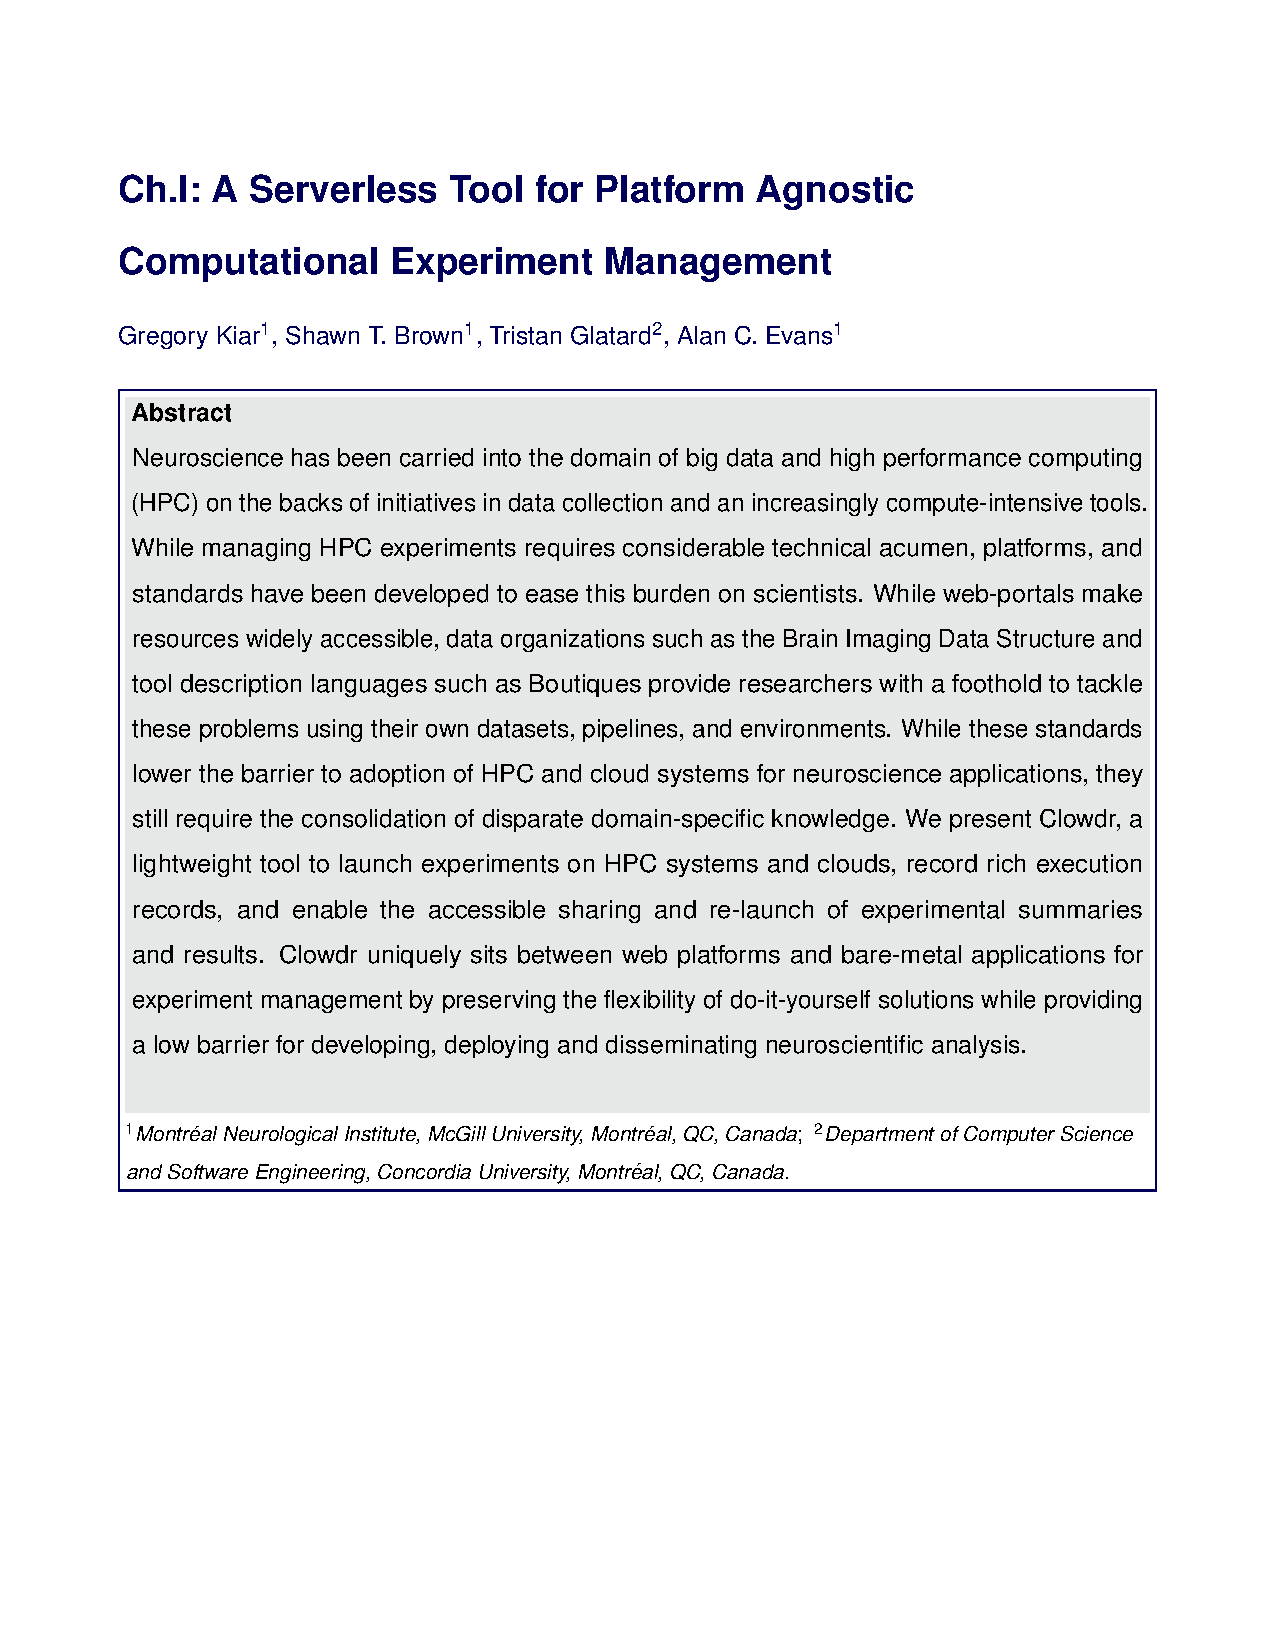
\includepdf[pages=-,pagecommand={\thispagestyle{fancy}},addtotoc={
     1,part,1,A Serverless Tool for Platform Agnostic Computational Experiment Management,ch1p1,   
     2,secnonum,2,\qquad\qquad Abstract,ch1p2,
     3,section,2,\qquad\qquad Introduction,ch1p2,
     4,section,2,\qquad\qquad Emergent Technologies in Reproducible Neuroscience,ch1p3,
     7,section,2,\qquad\qquad The Clowdr Microtool,ch1p6,
     10,section,2,\qquad\qquad Performing Experiments With Clowdr,ch1p9,
     13,section,2,\qquad\qquad Discussion,ch1p12}]
     {../chapter1/chapter1.pdf}
\clearpage

\phantomsection
\beginchapter{II}
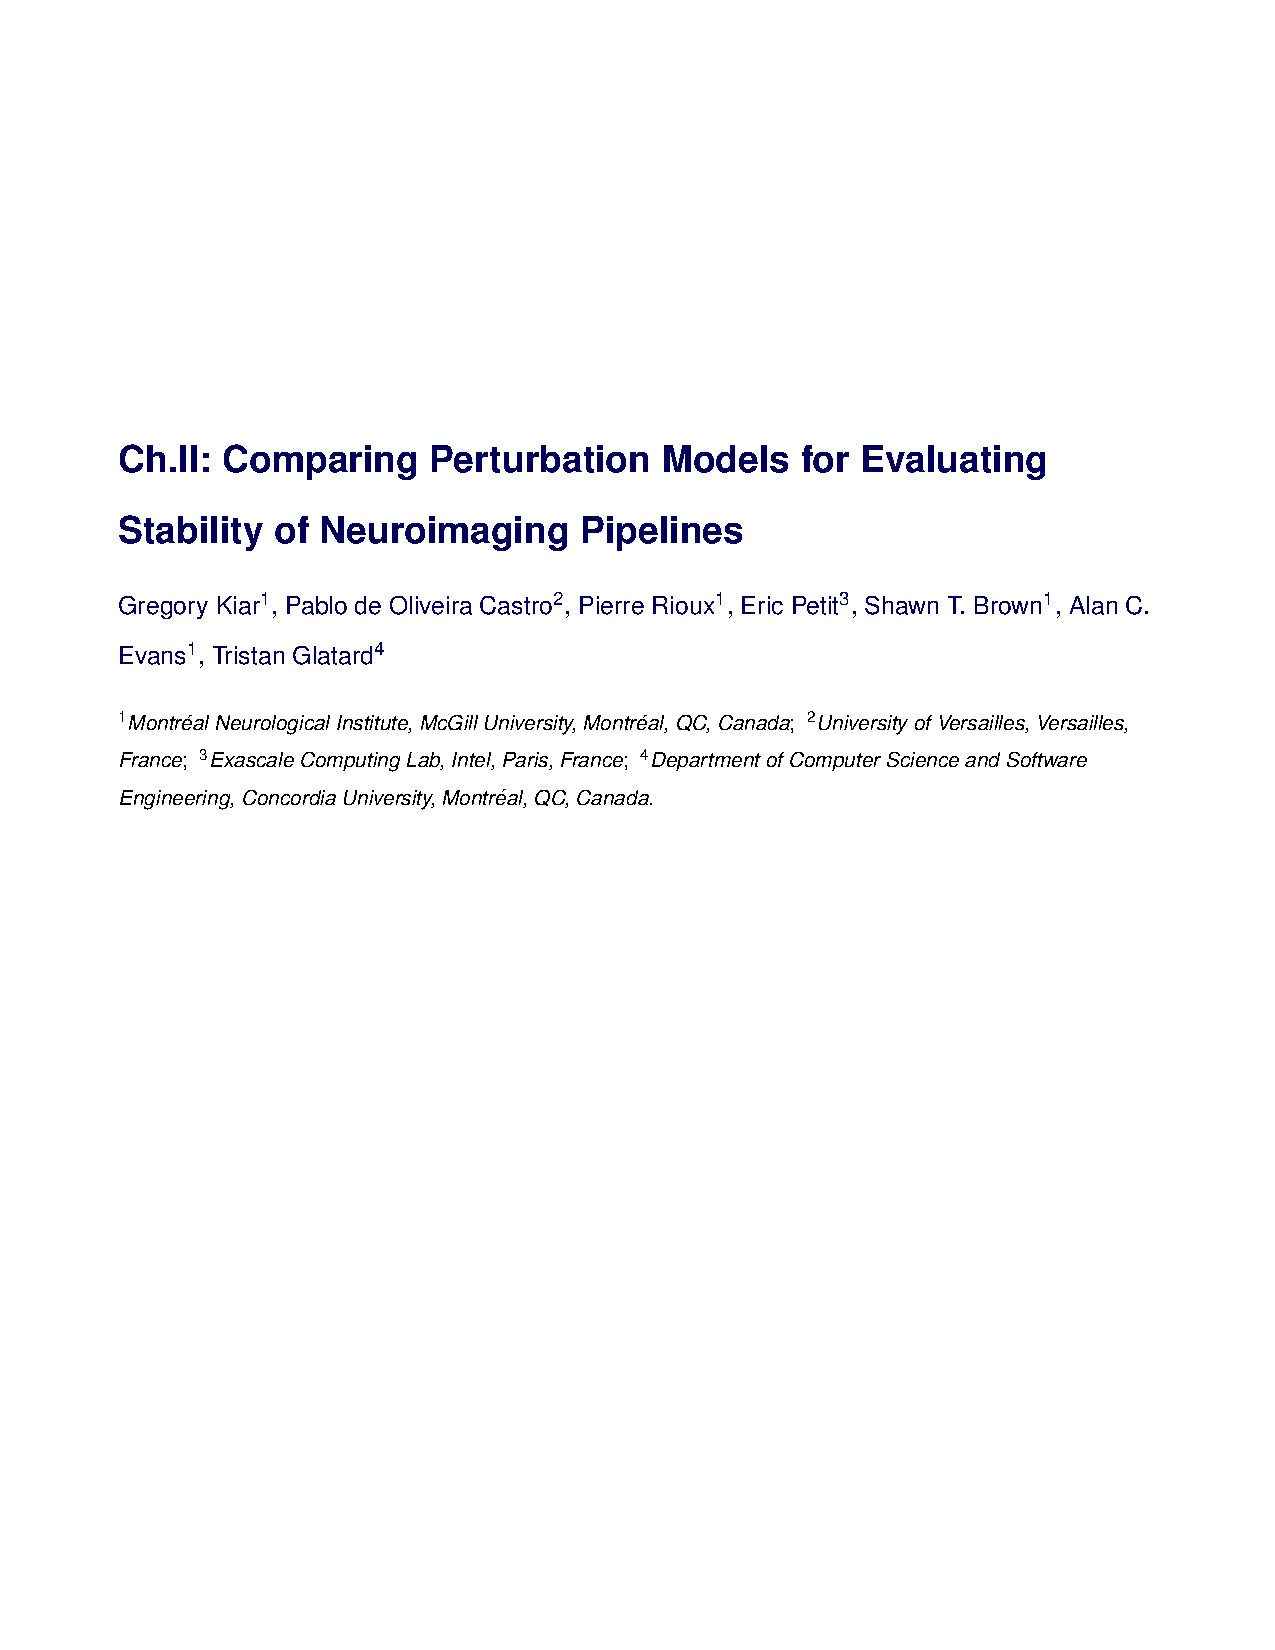
\includepdf[pages=-,pagecommand={\thispagestyle{fancy}},addtotoc={
     1,part,1,Comparing Perturbation Models for Evaluating Stability of Neuroimaging Pipelines,ch2p1,   
     2,secnonum,2,\qquad\qquad Abstract,ch2p2,
     3,section,2,\qquad\qquad Introduction,ch2p3,
     4,section,2,\qquad\qquad Methods,ch2p4,
     10,section,2,\qquad\qquad Results,ch2p10,
     15,section,2,\qquad\qquad Discussion,ch2p15,
     19,section,2,\qquad\qquad Conclusion,ch2p19}]
     {../chapter2/chapter2.pdf}
\clearpage

\phantomsection
\beginchapter{III}
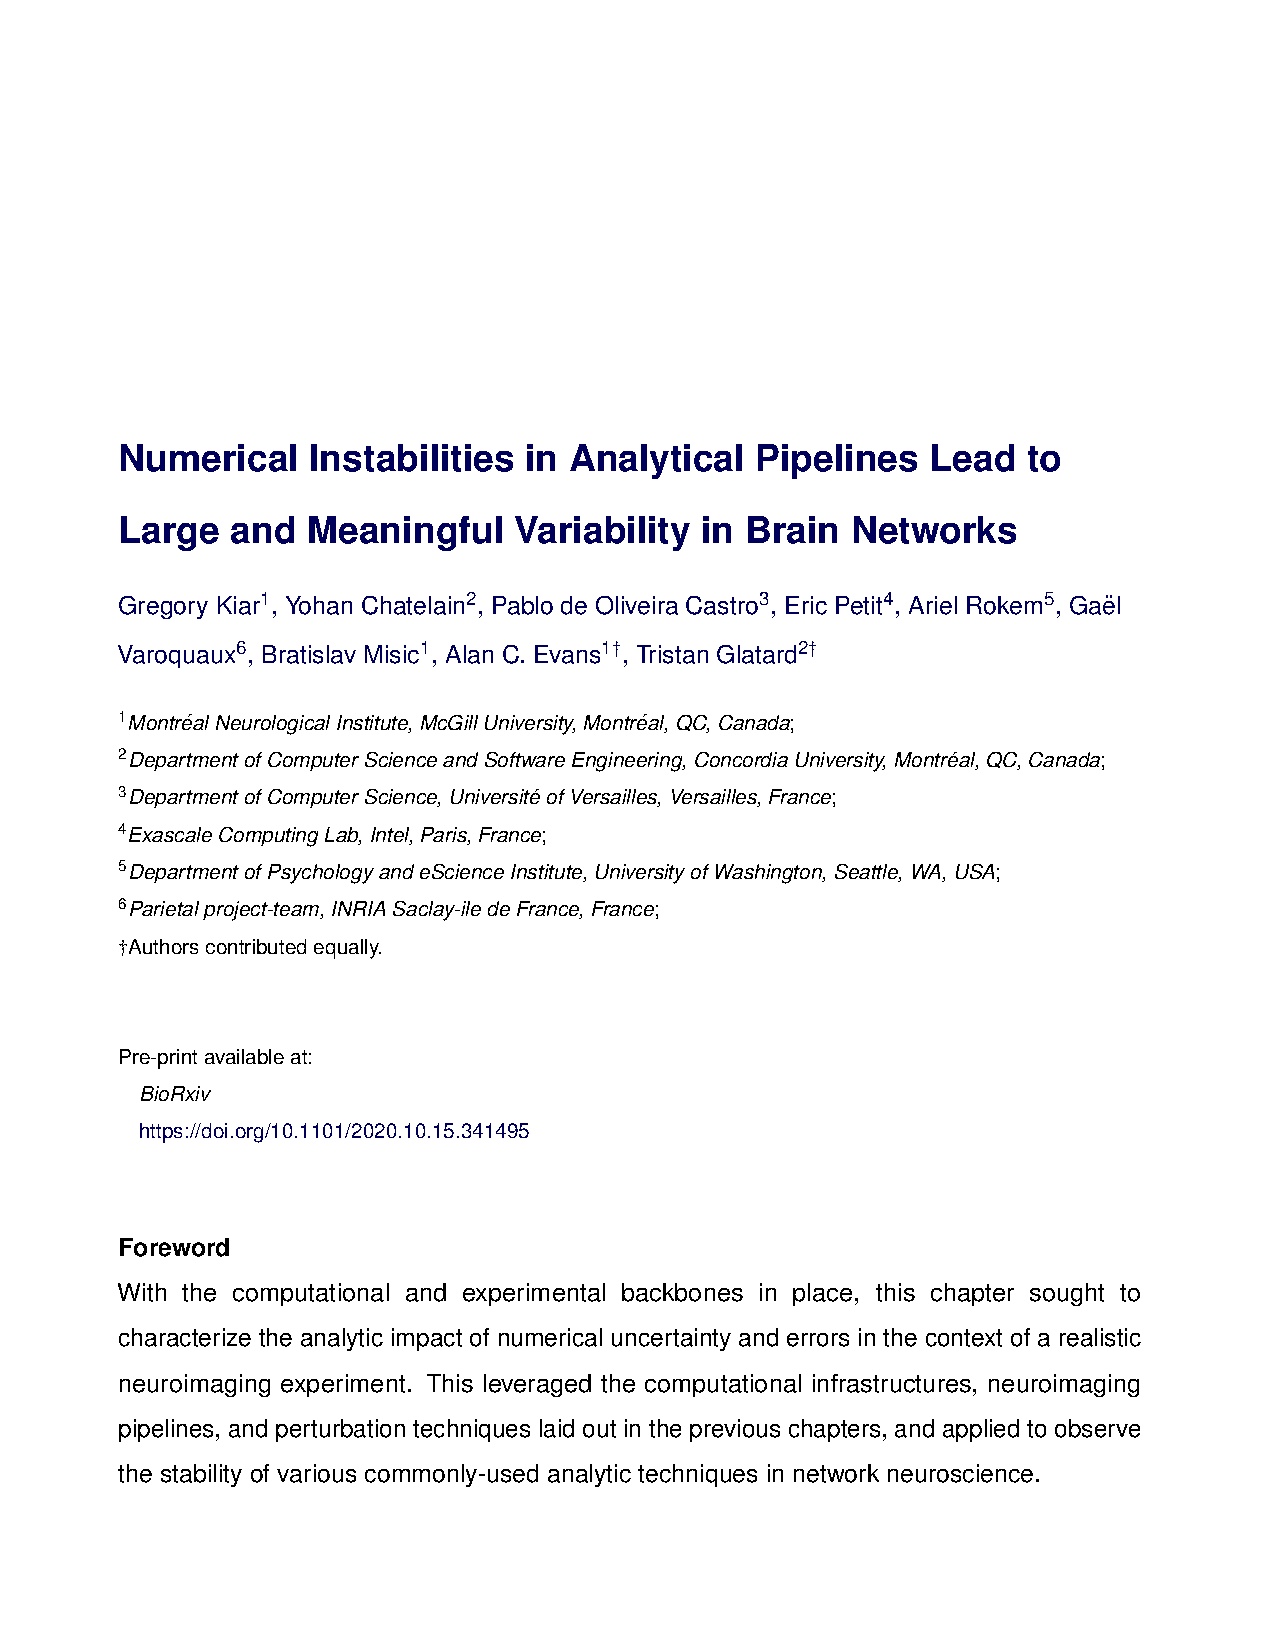
\includepdf[pages=-,pagecommand={\thispagestyle{fancy}},addtotoc={
     1,part,1,Numerical Instabilities in Analytical Pipelines Lead to Large and Meaningful \\ Variability in Brain Networks,ch3p1,
     2,secnonum,2,\qquad\qquad Abstract,ch3p2,
     3,section,2,\qquad\qquad Graphs Vary Widely With Perturbations,ch3p3,
     5,section,2,\qquad\qquad Subject-Specific Signal is Amplified While Off-Target Biases Are Reduced,ch3p5,
     7,section,2,\qquad\qquad {Distributions of Graph Statistics Are Reliable, But Individual Statistics Are Not},ch3p7,
     9,section,2,\qquad\qquad Uncertainty in Brain-Phenotype Relationships,ch3p9,
     10,section,2,\qquad\qquad Discussion,ch3p10,
     12,section,2,\qquad\qquad Materials \& Methods,ch3p12,
     22,supsec,2,\qquad\qquad Graph Correlation,ch3p22,
     23,supsec,2,\qquad\qquad Complete Discriminability Analysis,ch3p23,
     24,supsec,2,\qquad\qquad Univariate Graph Statistics,ch3p24}]
     {../chapter3/chapter3.pdf}

\phantomsection
\beginchapter{IV}
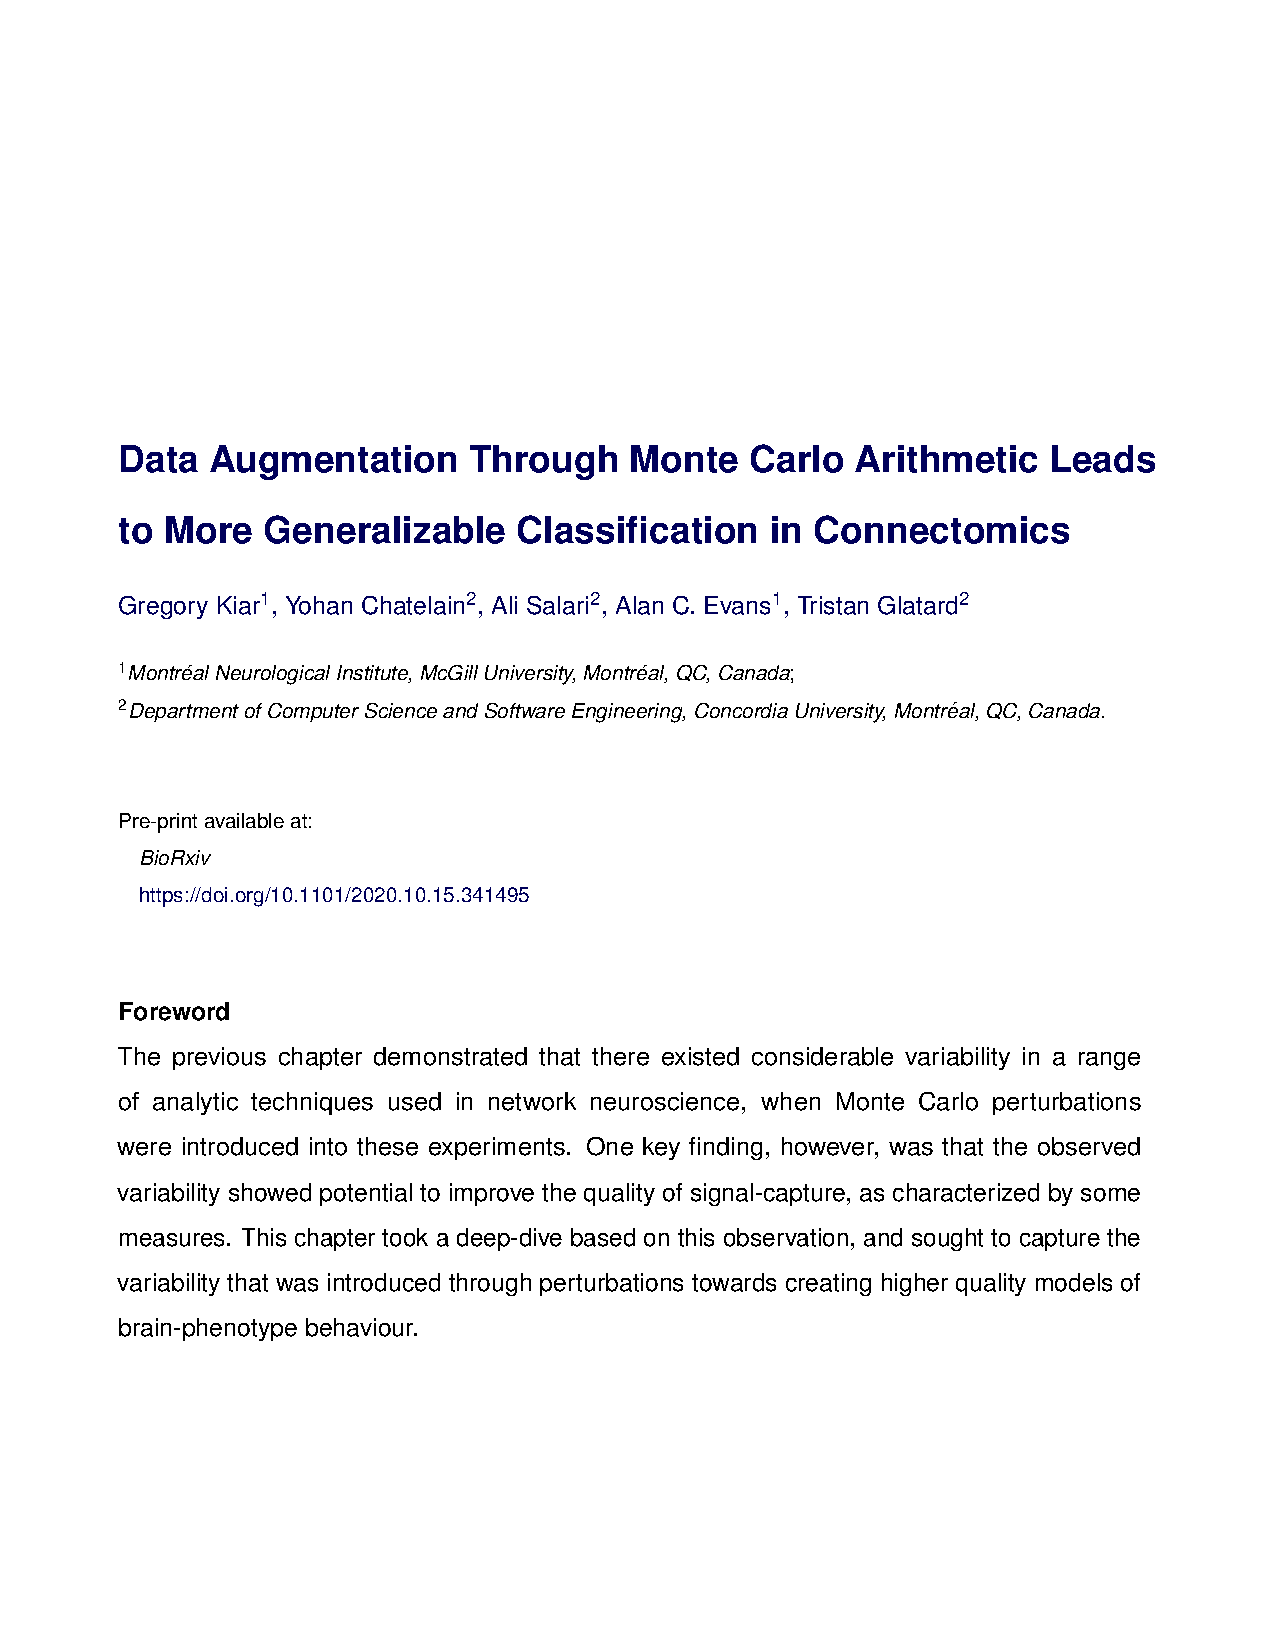
\includepdf[pages=-,pagecommand={\thispagestyle{fancy}},addtotoc={
     1,part,1,Data Augmentation Through Monte Carlo Arithmetic Leads to More Generalizable Classification in Connectomics,ch4p1,
     2,secnonum,2,\qquad\qquad Abstract,ch4p2,
     3,section,2,\qquad\qquad Introduction,ch4p3a,
     3,section,2,\qquad\qquad Materials \& Methods,ch4p3b,
     8,section,2,\qquad\qquad Results,ch4p8,
     13,section,2,\qquad\qquad Discussion,ch4p13,
     16,section,2,\qquad\qquad Conclusion,ch4p16}]
     {../chapter4/chapter4.pdf}
\twocolumn


%----------------------------------------------------------------------------------------
% Discussion and Wrap up
%----------------------------------------------------------------------------------------
\resetsections{2}
\phantomsection

\section{Discussion}
\begin{itemize}
\item Comparing and contrasting community variability
\item https://www.biorxiv.org/content/10.1101/2020.10.07.321083v1
\item NARPS
\item Expanding insights to other modalities and tool domains
\end{itemize}

\section{Conclusion \& Summary}
words

\section{References}
words

%----------------------------------------------------------------------------------------
%	REFERENCE LIST
%----------------------------------------------------------------------------------------
% \phantomsection
% \bibliographystyle{IEEEtran}
% \bibliography{gkiar_thesis}

%----------------------------------------------------------------------------------------
\end{document}
